\chapter{Numbers 26}

\begin{figure}
  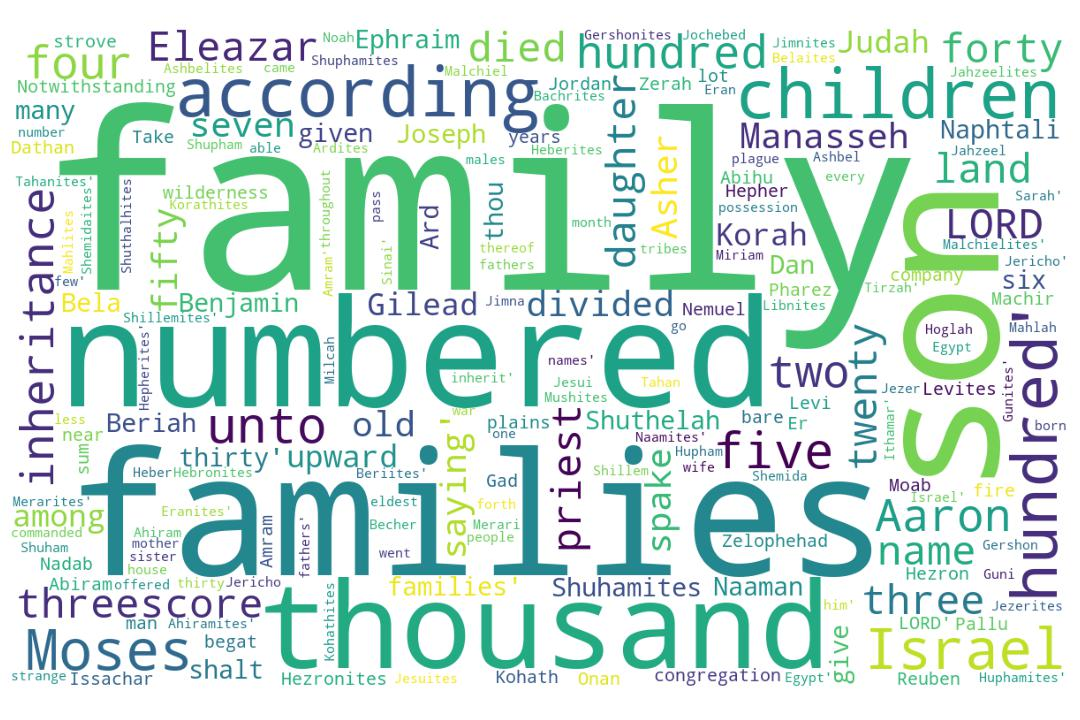
\includegraphics[width=\linewidth]{04OT-Numbers/Numbers26-WordCloud.jpg}
  \caption{Numbers 26 Word Cloud}
  \label{fig:Numbers 26 word Cloud}
\end{figure}

\marginpar{\scriptsize \centering \fcolorbox{bone}{lime}{\textbf{A GENERATION LATER}}\\ (Numbers 26)
\begin{compactenum}[I.][8]
    \item The \textbf{Priests} \index[scripture]{Numbers!Num 26:01}\index[scripture]{Numbers!Num 26:03}\index[scripture]{Numbers!Num 26:63}\index[scripture]{Numbers!Num 26:64} (Numbers 26:1, 3, 63, 64)
    \item The \textbf{Plague} \index[scripture]{Numbers!Num 26:01} (Numbers 26:1)
    \item The \textbf{Plains} of Moab \index[scripture]{Numbers!Num 26:03}\index[scripture]{Numbers!Num 26:64} (Numbers 26:3, 64)
    \item The \textbf{People} 
    \item The \textbf{Population} \index[scripture]{Numbers!Num 26:12--54} (Numbers 26:12--54) Note the differences in population among the various tribes. Simeon loses almost 63\% of its people, while some of the tribes grow substantially.
    \item The \textbf{Possessions} \index[scripture]{Numbers!Num 26:56} (Numbers 26:56)
    \item A \textbf{Preview} 
\end{compactenum}}

%%%%%%%%%%%%%%%%%%%%%%%%%%%%%%%%%%
%%%%%%%%%%%%%%%%%%%%%%%%%%%%%%%%%%
\footnote{\textcolor[rgb]{0.00,0.25,0.00}{\hyperlink{TOC}{Return to end of Table of Contents.}}}\footnote{\href{https://audiobible.com/bible/numbers_26.html}{\textcolor[cmyk]{0.99998,1,0,0}{Numbers 26 Audio}}}\textcolor[cmyk]{0.99998,1,0,0}{And it came to pass after the plague, that the LORD spake unto Moses and unto Eleazar the son of Aaron the priest, saying,}
[2] \textcolor[cmyk]{0.99998,1,0,0}{Take the sum of all the congregation of the children of Israel, from twenty years old and upward, throughout their fathers' house, all that are able to go to war in Israel.}
[3] \textcolor[cmyk]{0.99998,1,0,0}{And Moses and Eleazar the priest spake with them in the plains of Moab by Jordan \emph{near} Jericho, saying,}
[4] \textcolor[cmyk]{0.99998,1,0,0}{\emph{Take} \emph{the} \emph{sum} \emph{of} \emph{the} \emph{people}, from twenty years old and upward; as the LORD commanded Moses and the children of Israel, which went forth out of the land of Egypt.}\\
\\
\P \textcolor[cmyk]{0.99998,1,0,0}{Reuben, the eldest son of Israel: the children of Reuben; Hanoch, \emph{of} \emph{whom} \emph{cometh} the family of the Hanochites: of Pallu, the family of the Palluites:}
[6] \textcolor[cmyk]{0.99998,1,0,0}{Of Hezron, the family of the Hezronites: of Carmi, the family of the Carmites.}
[7] \textcolor[cmyk]{0.99998,1,0,0}{These \emph{are} \fcolorbox{bone}{bone}{the familes} of the Reubenites: and they that were numbered of them were forty and three \fcolorbox{bone}{bone}{thousand and} seven hundred and thirty.}
[8] \textcolor[cmyk]{0.99998,1,0,0}{And the sons of Pallu; Eliab.}
[9] \textcolor[cmyk]{0.99998,1,0,0}{And the sons of Eliab; Nemuel, and Dathan, and Abiram. This \emph{is} \emph{that} Dathan and Abiram, \emph{which} \emph{were} famous in the congregation, who strove against Moses and against Aaron in the company of Korah, when they strove against the LORD:}\footnote{\textbf{Numbers 16:1-3} - Now Korah, the son of Izhar, the son of Kohath, the son of Levi, and Dathan and Abiram, the sons of Eliab, and On, the son of Peleth, sons of Reuben, took men: [2] And they rose up before Moses, with certain of the children of Israel, two hundred and fifty princes of the assembly, famous in the congregation, men of renown: [3] And they gathered themselves together against Moses and against Aaron, and said unto them, Ye take too much upon you, seeing all the congregation are holy, every one of them, and the LORD is among them: wherefore then lift ye up yourselves above the congregation of the LORD?}\footnote{\textbf{Deuteronomy 11:6} - And what he did unto Dathan and Abiram, the sons of Eliab, the son of Reuben: how the earth opened her mouth, and swallowed them up, and their households, and their tents, and all the substance that was in their possession, in the midst of all Israel:}\footnote{\textbf{Psalm 106:17} - The earth opened and swallowed up Dathan, and covered the company of Abiram.}
[10] \textcolor[cmyk]{0.99998,1,0,0}{And the earth opened her mouth, and swallowed them up together with Korah, when that company died, what time the fire devoured two hundred and fifty men: and they became a sign.}
[11] \textcolor[cmyk]{0.99998,1,0,0}{Notwithstanding the children of Korah died not.}\\
\\
\P \textcolor[cmyk]{0.99998,1,0,0}{The sons of Simeon after their families: of Nemuel, the family of the Nemuelites: of Jamin, the family of the Jaminites: of Jachin, the family of the Jachinites:}
[13] \textcolor[cmyk]{0.99998,1,0,0}{Of Zerah, the family of the Zarhites: of Shaul, the family of the Shaulites.}
[14] \textcolor[cmyk]{0.99998,1,0,0}{These \emph{are} \fcolorbox{bone}{bone}{the familes} of the Simeonites, twenty and two \fcolorbox{bone}{bone}{thousand and} two hundred.}\\
\\
\P \textcolor[cmyk]{0.99998,1,0,0}{The children of Gad after their families: of Zephon, the family of the Zephonites: of Haggi, the family of the Haggites: of Shuni, the family of the Shunites:}
[16] \textcolor[cmyk]{0.99998,1,0,0}{Of Ozni, the family of the Oznites: of Eri, the family of the Erites:}
[17] \textcolor[cmyk]{0.99998,1,0,0}{Of Arod, the family of the Arodites: of Areli, the family of the Arelites.}
[18] \textcolor[cmyk]{0.99998,1,0,0}{These \emph{are} \fcolorbox{bone}{bone}{the familes} of the children of Gad according to those that were numbered of them, forty \fcolorbox{bone}{bone}{thousand and} five hundred.}\\
\\
\P \textcolor[cmyk]{0.99998,1,0,0}{The sons of Judah \emph{were} Er and Onan: and Er and Onan died in the land of Canaan.}
[20] \textcolor[cmyk]{0.99998,1,0,0}{And the sons of Judah after their families were; of Shelah, the family of the Shelanites: of Pharez, the family of the Pharzites: of Zerah, the family of the Zarhites.}
[21] \textcolor[cmyk]{0.99998,1,0,0}{And the sons of Pharez were; of Hezron, the family of the Hezronites: of Hamul, the family of the Hamulites.}
[22] \textcolor[cmyk]{0.99998,1,0,0}{These \emph{are} \fcolorbox{bone}{bone}{the familes} of Judah according to those that were numbered of them, threescore and sixteen \fcolorbox{bone}{bone}{thousand and} five hundred.}\\
\\
\P \textcolor[cmyk]{0.99998,1,0,0}{\emph{Of} the sons of Issachar after their families: \emph{of} Tola, the family of the Tolaites: of Pua, the family of the Punites:}
[24] \textcolor[cmyk]{0.99998,1,0,0}{Of Jashub, the family of the Jashubites: of Shimron, the family of the Shimronites.}
[25] \textcolor[cmyk]{0.99998,1,0,0}{These \emph{are} \fcolorbox{bone}{bone}{the familes} of Issachar according to those that were numbered of them, threescore and four \fcolorbox{bone}{bone}{thousand and} three hundred.}\\
\\
\P \textcolor[cmyk]{0.99998,1,0,0}{\emph{Of} the sons of Zebulun after their families: of Sered, the family of the Sardites: of Elon, the family of the Elonites: of Jahleel, the family of the Jahleelites.}
[27] \textcolor[cmyk]{0.99998,1,0,0}{These \emph{are} \fcolorbox{bone}{bone}{the familes} of the Zebulunites according to those that were numbered of them, threescore \fcolorbox{bone}{bone}{thousand and} five hundred.}\\
\\
\P \textcolor[cmyk]{0.99998,1,0,0}{The sons of Joseph after their families \emph{were} Manasseh and Ephraim.}
[29] \textcolor[cmyk]{0.99998,1,0,0}{Of the sons of Manasseh: of Machir, the family of the Machirites: and Machir begat Gilead: of Gilead \emph{come} the family of the Gileadites.}
[30] \textcolor[cmyk]{0.99998,1,0,0}{These \emph{are} the sons of Gilead: \emph{of} Jeezer, the family of the Jeezerites: of Helek, the family of the Helekites:}
[31] \textcolor[cmyk]{0.99998,1,0,0}{And \emph{of} Asriel, the family of the Asrielites: and \emph{of} Shechem, the family of the Shechemites:}
[32] \textcolor[cmyk]{0.99998,1,0,0}{And \emph{of} Shemida, the family of the Shemidaites: and \emph{of} Hepher, the family of the Hepherites.}
[33] \textcolor[cmyk]{0.99998,1,0,0}{And Zelophehad the son of Hepher had no sons, but daughters: and the names of the daughters of Zelophehad \emph{were} Mahlah, and Noah, Hoglah, Milcah, and Tirzah.}\footnote{\textbf{Numbers 36:2-3} - And they said, The LORD commanded my lord to give the land for an inheritance by lot to the children of Israel: and my lord was commanded by the LORD to give the inheritance of Zelophehad our brother unto his daughters. [3] And if they be married to any of the sons of the other tribes of the children of Israel, then shall their inheritance be taken from the inheritance of our fathers, and shall be put to the inheritance of the tribe whereunto they are received: so shall it be taken from the lot of our inheritance.}
[34] \textcolor[cmyk]{0.99998,1,0,0}{These \emph{are} \fcolorbox{bone}{bone}{the familes} of Manasseh, and those that were numbered of them, fifty and two \fcolorbox{bone}{bone}{thousand and} seven hundred.}\\
\\
\P \textcolor[cmyk]{0.99998,1,0,0}{These \emph{are} the sons of Ephraim after their families: of Shuthelah, the family of the Shuthalhites: of Becher, the family of the Bachrites: of Tahan, the family of the Tahanites.}
[36] \textcolor[cmyk]{0.99998,1,0,0}{And these \emph{are} the sons of Shuthelah: of Eran, the family of the Eranites.}
[37] \textcolor[cmyk]{0.99998,1,0,0}{These \emph{are} \fcolorbox{bone}{bone}{the familes} of the sons of Ephraim according to those that were numbered of them, thirty and two \fcolorbox{bone}{bone}{thousand and} five hundred. These \emph{are} the sons of Joseph after their families.}\\
\\
\P \textcolor[cmyk]{0.99998,1,0,0}{The sons of Benjamin after their families: of Bela, the family of the Belaites: of Ashbel, the family of the Ashbelites: of Ahiram, the family of the Ahiramites:}
[39] \textcolor[cmyk]{0.99998,1,0,0}{Of Shupham, the family of the Shuphamites: of Hupham, the family of the Huphamites.}
[40] \textcolor[cmyk]{0.99998,1,0,0}{And the sons of Bela were Ard and Naaman: \emph{of} \emph{Ard}, the family of the Ardites: \emph{and} of Naaman, the family of the Naamites.}
[41] \textcolor[cmyk]{0.99998,1,0,0}{These \emph{are} the sons of Benjamin after their families: and they that were numbered of them \emph{were} forty and five \fcolorbox{bone}{bone}{thousand and} six hundred.}\\
\\
\P \textcolor[cmyk]{0.99998,1,0,0}{These \emph{are} the sons of Dan after their families: of Shuham, the family of the Shuhamites. These \emph{are} \fcolorbox{bone}{bone}{the familes} of Dan after their families.}
[43] \textcolor[cmyk]{0.99998,1,0,0}{All \fcolorbox{bone}{bone}{the familes} of the Shuhamites, according to those that were numbered of them, \emph{were} threescore and four \fcolorbox{bone}{bone}{thousand and} four hundred.}\\
\\
\P \textcolor[cmyk]{0.99998,1,0,0}{\emph{Of} the children of Asher after their families: of Jimna, the family of the Jimnites: of Jesui, the family of the Jesuites: of Beriah, the family of the Beriites.}
[45] \textcolor[cmyk]{0.99998,1,0,0}{Of the sons of Beriah: of Heber, the family of the Heberites: of Malchiel, the family of the Malchielites.}
[46] \textcolor[cmyk]{0.99998,1,0,0}{And the name of the daughter of Asher \emph{was} Sarah.}
[47] \textcolor[cmyk]{0.99998,1,0,0}{These \emph{are} \fcolorbox{bone}{bone}{the familes} of the sons of Asher according to those that were numbered of them; \emph{who} \emph{were} fifty and three \fcolorbox{bone}{bone}{thousand and} four hundred.}\\
\\
\P \textcolor[cmyk]{0.99998,1,0,0}{\emph{Of} the sons of Naphtali after their families: of Jahzeel, the family of the Jahzeelites: of Guni, the family of the Gunites:}
[49] \textcolor[cmyk]{0.99998,1,0,0}{Of Jezer, the family of the Jezerites: of Shillem, the family of the Shillemites.}
[50] \textcolor[cmyk]{0.99998,1,0,0}{These \emph{are} \fcolorbox{bone}{bone}{the familes} of Naphtali according to their families: and they that were numbered of them \emph{were} forty and five \fcolorbox{bone}{bone}{thousand and} four hundred.}
[51] \textcolor[cmyk]{0.99998,1,0,0}{These \emph{were} the numbered of the children of Israel, six hundred \fcolorbox{bone}{bone}{thousand and} a thousand seven hundred and thirty.}\\
\\
\P \textcolor[cmyk]{0.99998,1,0,0}{And the LORD spake unto Moses, saying,}
[53] \textcolor[cmyk]{0.99998,1,0,0}{Unto these the land shall be divided for an inheritance according to the number of names.}
[54] \textcolor[cmyk]{0.99998,1,0,0}{To many thou shalt give the more inheritance, and to few thou shalt give the less inheritance: to every one shall his inheritance be given according to those that were numbered of him.}
[55] \textcolor[cmyk]{0.99998,1,0,0}{Notwithstanding the land shall be divided by lot: according to the names of the tribes of their fathers they shall inherit.}
[56] \textcolor[cmyk]{0.99998,1,0,0}{According to the lot shall the possession thereof be divided between many and few.}\\
\\
\P \textcolor[cmyk]{0.99998,1,0,0}{And these \emph{are} they that were numbered of the Levites after their families: of Gershon, the family of the Gershonites: of Kohath, the family of the Kohathites: of Merari, the family of the Merarites.}
[58] \textcolor[cmyk]{0.99998,1,0,0}{These \emph{are} \fcolorbox{bone}{bone}{the familes} of the Levites: the family of the Libnites, the family of the Hebronites, the family of the Mahlites, the family of the Mushites, the family of the Korathites. And Kohath begat Amram.}
[59] \textcolor[cmyk]{0.99998,1,0,0}{And the name of Amram's wife \emph{was} Jochebed, the daughter of Levi, whom \emph{her} \emph{mother} bare to Levi in Egypt: and she bare unto Amram Aaron and Moses, and Miriam their sister.}
[60] \textcolor[cmyk]{0.99998,1,0,0}{And unto Aaron was born Nadab, and Abihu, Eleazar, and Ithamar.}
[61] \textcolor[cmyk]{0.99998,1,0,0}{And Nadab and Abihu died, when they offered strange fire before the LORD.}\footnote{\textbf{Numbers 3:4} - And Nadab and Abihu died before the LORD, when they offered strange fire before the LORD, in the wilderness of Sinai, and they had no children: and Eleazar and Ithamar ministered in the priest’s office in the sight of Aaron their father.}\footnote{\textbf{Numbers 10:1-2} - And Nadab and Abihu, the sons of Aaron, took either of them his censer, and put fire therein, and put incense thereon, and offered strange fire before the LORD, which he commanded them not. [2] And there went out fire from the LORD, and devoured them, and they died before the LORD.}
[62] \textcolor[cmyk]{0.99998,1,0,0}{And those that were numbered of them were twenty and three thousand, all males from a month old and upward: for they were not numbered among the children of Israel, because there was no inheritance given them among the children of Israel.}
[63] \textcolor[cmyk]{0.99998,1,0,0}{These \emph{are} they that were numbered by Moses and Eleazar the priest, who numbered the children of Israel in the plains of Moab by Jordan \emph{near} Jericho.}
[64] \textcolor[cmyk]{0.99998,1,0,0}{But among these there was not a man of them whom Moses and Aaron the priest numbered, when they numbered the children of Israel in the wilderness of Sinai.}
[65] \textcolor[cmyk]{0.99998,1,0,0}{For the LORD had said of them, They shall surely die in the wilderness. And there was not left a man of them, save Caleb the son of Jephunneh, and Joshua the son of Nun.}